% Modelo de Dissertação em Latex para o PPG em Engenharia Mecânica da UERJ
% Este modelo foi adaptado da versão disponibilizada no site da Engenharia Elétrica da UERJ
% http://www.pel.uerj.br/publico/Modelo_LaTeX_Dissertacao_UERJ.rar
% http://www.pel.uerj.br/defesas/
%
% Utilizei o WinEdt 6.0 com Miktex 2.9
%
% Para gerar o PDF usei a opção PDFTeXfy com o documento [masterthesis.tex] aberto e em foco.
%
% Não consegui usar as figuras em EPS como o modelo original. Usei PNG e JPG sem problemas.
%
% Felipe M. - 20/06/2012
%

% Modificações e adaptações ao modelo da UFPE feitas por João Cordeiro.
% Versão original disponibilizada como template do latex.
% Este modelo foi criado para servir de exemplo de formato, não devendo seu código ser
% utilizado como referência de formatação.
% PLAIN: O código é uma adaptação de uma adaptação. Funciona, mas está cheio de gambiarras.
%
% João Cordeiro - 05/03/2019
%

\documentclass[a4paper,12pt,oneside,openany,table,xcdraw]{uerj}

\usepackage[portuguese]{babel}
%\usepackage[latin1]{inputenc}
\usepackage[utf8]{inputenc}
\usepackage{enumerate}
\usepackage{cite}
\usepackage{epsf,epsfig,psfig}
\usepackage{pagina}
\usepackage{indentfirst}
\usepackage{theorem}
\usepackage{fancyhdr}
\usepackage{setspace}
\usepackage{boxedminipage}
\usepackage{float}
\usepackage{makeidx}
\usepackage{amsmath}
\usepackage{mathtools}
\usepackage[hidelinks]{hyperref}
\usepackage{todonotes}
\usepackage{caption}
\usepackage{graphicx}
\usepackage{multirow}
\usepackage{blindtext}
 \usepackage{siunitx}

\usepackage{amssymb}
\usepackage{mathtools}
\usepackage{relsize}

\usepackage{charter}
\usepackage{environ}
\usepackage{tikz}
\usetikzlibrary{calc,matrix}

\usepackage{filecontents}

\usepackage[usenames,dvipsnames]{xcolor}

\usepackage{tcolorbox}
\usepackage{tabularx}
\usepackage{array}
\usepackage{colortbl}
\tcbuselibrary{skins}

\newcolumntype{Y}{>{\raggedleft\arraybackslash}X}

\tcbset{tab1/.style={enhanced, fonttitle=\bfseries,fontupper=\scriptsize,
colback=SpringGreen!05!white,colframe=LimeGreen!15!black,colbacktitle=YellowGreen!15!white,
coltitle=black,center title}}

\usepackage{graphicx}

% Comando para remover o rodapé(footer)
\usepackage{fancyhdr}
\pagestyle{fancy}
% your header and footer code
\fancyfoot[C]{}

% Bilibotecas para referências 
\usepackage{cite}
\usepackage[super]{natbib}

\usepackage[hang, small,labelfont=bf,up,textfont=it,up]{caption}
\usepackage{listings}

% Comandos importantes para tornar section/subsection em negrito %
\usepackage{titlesec}
\titleformat{\section}    
       {\renewcommand\rmdefault{lmr}\fontsize{12}{17}\bfseries}{\thesection}{1em}{}

\titleformat{\subsection}    
       {\renewcommand\rmdefault{lmr}\fontsize{12}{17}\bfseries\itshape}{\thesubsection}{1em}{}

%\usepackage[Bjornstrup]{fncychap}

\usepackage[T1]{fontenc}
\usepackage{titlesec, blindtext, color}
\definecolor{gray75}{gray}{0.75}
\titlespacing*{\chapter}{0pt}{-25pt}{30pt}
\titleformat{\chapter}[hang]{\Huge\bfseries}{\thechapter\hsp\textcolor{gray75}{|}\hsp}{0pt}{\Huge\bfseries}

\newtheorem{deff}{Definição}[section]
\numberwithin{equation}{chapter}

\theoremstyle{plain}

\newcommand*{\captionsource}[3]{%
    \caption{\label{#1}#2.}
    \vspace{-0.3cm}
    \caption*{Fonte: #3.}
}

\fancypagestyle{references}{%
  \lhead{Referências}
  \chead{}
  \rhead{}
  \rhead{\thepage}
}


\fancypagestyle{timeline}{%
  \lhead{Cronograma}
  \chead{}
  \rhead{}
  \rhead{\thepage}
}

\renewcommand\rmdefault{lmr}

\begin{document}

\hypersetup{
    colorlinks,
    citecolor=black,
    filecolor=black,
    linkcolor=black,
    urlcolor=black,
    linktoc=all
}
% Infos do projeto
%

\pagestyle{empty}

\newcommand{\thedepartment}{Instituto de Ciências Exatas}
\newcommand{\thecourse}{Departamento de Física}
\newcommand{\thetype}{Relatório de Iniciação Científica}
\newcommand{\thestudent}{Micael Davi Lima de Oliveira}
\newcommand{\theadvisor}{Prof. Dr. Kelson Mota Teixeira de Oliveira}
\newcommand{\thecity}{Manaus}

% \thispagestyle{empty}\listoftodos\pagebreak
\thispagestyle{empty}\newcommand*{\themonth}{\ifthenelse{\the\month < 2}{Janeiro }
                  {\ifthenelse{\the\month < 3}{Fevereiro }
                  {\ifthenelse{\the\month < 4}{Março }
                  {\ifthenelse{\the\month < 5}{Abril }
                  {\ifthenelse{\the\month < 6}{Maio }
                  {\ifthenelse{\the\month < 7}{Junho }
                  {\ifthenelse{\the\month < 8}{Julho }
                  {\ifthenelse{\the\month < 9}{Agosto }
                  {\ifthenelse{\the\month < 10}{Setembro }
                  {\ifthenelse{\the\month < 11}{Outubro }
                  {\ifthenelse{\the\month < 12}{Novembro }{Dezembro }}}}}}}}}}}}
                  

\begin{titlepage}
\begin{center}

	\vspace{-0.5cm}

  \begin{figure}[hbt!]
		\begin{center}
		   \includegraphics[scale=0.15]{Figuras/MarcaUFAM.png}
		\end{center}
	\end{figure}
% 	\vspace{-4cm}

  \large{Universidade Federal do Amazonas}\\
  \large{Pró-Reitoria de Pesquisa e Pós-Graduação}\\
  \large{Departamento de Apoio à Pesquisa}\\
  \large{Programa Institucional de Iniciação Científica}\\

  \hspace{2cm}\large{}\\
  \hspace{2cm}\large{}\\
  
  \hspace{2cm}\large{}\\
  \hspace{2cm}\large{}\\

  \large\textbf{Predição de novos fármacos antagonistas de interleucina IL-6 no tratamento de transtorno depressivo}

  \hspace{2cm}\large{}\\
  \hspace{2cm}\large{}\\
  
  \par  
  \large{\thestudent}\\
  
  \hspace{2cm}\large{}\\
  \hspace{2cm}\large{}\\
 
  \par\vfill
  Manaus - AM \\ 2020

\end{center}
\end{titlepage}
\pagebreak\thispagestyle{empty}\begin{center}

\text{Micael Davi Lima de Oliveira} 

% \vfill
\vspace{2cm}

\textbf{Predição de novos fármacos antagonistas de interleucina IL-6 no tratamento de transtorno depressivo}

\vspace{6.0cm}

% \begin{figure}[hbt!]
% \begin{center}
% \includegraphics[width=10.48cm]{./01_Pre_textuais/logo_ufpe.png}
% \end{center}
% \end{figure}

\begin{flushright}
\parbox{8cm}{
\singlespacing{\begin{hyphenrules}{nohyphenation}
Proposta de pesquisa apresentada à Comissão Científica da FAPEAM, como requisito parcial para inscrição no Programa de Bolsas de Iniciação Científica. \\
\end{hyphenrules}}}

Área de concentração: Física Atômica e Molecular \\
Opção: Física Biomolecular

% \linebreak 
\vspace{1.0cm}
\textbf{Orientador:} \theadvisor\\
\textbf{Colaborador:} Prof. Dr. Puspitapallab Chaudhuri
\end{flushright}

\par\vfill
%\vspace{2cm}

Manaus - AM\\2020

\end{center}

\pagebreak\thispagestyle{empty}\thispagestyle{empty}

\vspace*{200mm}
\begin{flushright}
	\textit{Dedicado a todos acometidos pelo Transtorno Depressivo e que já não mais conseguem ver uma luz ao final do túnel.}
\end{flushright}


\pagebreak\thispagestyle{empty}\begin{flushleft}
\Huge\bfseries{Agradecimentos} 
\end{flushleft}

\vspace{0.5cm}

Agradeço muito a Deus, por me dar forças e esperança em viver. Ainda que eu não mereça tamanho amor, me fortalece nos momentos de tristeza. \\

Aos meus pais, com o mais profundo amor e sincera gratidão. \\

Aos professores Kelson Mota e Puspitapallab, cujo conhecimento transmitido foi imprescindível para a realização desta pesquisa. \\

\pagebreak\thispagestyle{empty}\begin{flushleft}
\Huge\bfseries{Resumo} 
\end{flushleft}

\vspace{0.25cm}
$\!$
\noindent

\noindent{\small\textit{OLIVEIRA, M. D. L. \textbf{Predição de novos fármacos antagonistas de interleucina IL-6 no tratamento de transtorno depressivo}. 2020. 45 p. Iniciação Científica - Departamento de Física, Universidade Federal do Amazonas, Manaus, 2020.}} \\

O Transtorno Depressivo Maior(MDD) e seus subtipos já acometem mais de 300 milhões de pessoas no mundo, conforme um levantamento da OMS em 2017. Estima-se que de 30-50$\%$ dos pacientes não apresentam remissão completa dos sintomas. Diante disto, o impacto da depressão na humanidade não pode ser negligenciado. Diversas pesquisas sugerem que a depressão é acompanhada de desregulação imunológica e ativação do sistema de resposta inflamatória(IRS). Altas taxas de resistência ao tratamento podem estar correlacionadas aos inúmeros mecanismos da fisiopatologia, como aumento da atividade inflamatória, que mantém-se inalterado pela grande parte dos atuais antidepressivos. Níveis elevados de citocinas pro-inflamatórias(TNF-$\alpha$, IL-1, IL-6) e indução de suas vias de sinalização(sgp80, STAT3, JAK) foram detectados no cérebro e no sangue periférico em pacientes acometidos pela depressão. 

\vspace{1cm}

\hspace{-1.3cm}\textbf{Palavras-chave:} Docking molecular, IL-6, trans-sinalização, antidepressivos.
\pagebreak\thispagestyle{empty}\begin{flushleft}
\Huge\bfseries{Abstract} 
\end{flushleft}

\vspace{0.5cm}
$\!$
\noindent

\noindent{\small\textit{OLIVEIRA, M. D. L. \textbf{Prediction of new IL-6 interleukin antagonist drugs in the treatment of depressive disorder}. 2020. 45 p. Scientific Iniciation - Departament of Physics, Federal University of Amazonas, Manaus, 2020.}} \\

\vspace{1cm}

\hspace{-1.3cm} \textbf{Keywords:} Molecular docking, IL-6, trans-signaling, antidepressants.

\pagebreak

\def\listtablename{Lista de Figuras}\listoffigures
\def\listtablename{Lista de Tabelas}\listoftables
\chapter*{Lista de Abreviaturas e Siglas}

\textbf{ADMET} \\  Absorção, distribuição, metabolismo, excreção e toxicidade, do inglês ``Absorption, distribution, metabolism, excretion and toxicity" \\

\textbf{B3YLP} \\ Funcional híbrido de troca de Becke, chamado B3, combinado com o funcional de correlação, denominado LYP (Lee, Yang e Parr). \\

\textbf{CADD}  \\  Descoberta de medicamentos assistida por computador, do inglês ``Computer-Aided Drug Discovery" \\

\textbf{CNC} \\  Sistema Nervoso Central, do inglês ``Central Nervous System" \\

\textbf{CRH/CRF} \\  Hormônio Liberador de Corticotrofina, do inglês ``Corticotropin-Releasing Hormone" \\

\textbf{DFT} \\    Teoria do Funcional da Densidade, do inglês ``Density Functional Theory" \\ 

\textbf{DSM-5} \\  Manual Diagnóstico e Estatístico de Transtornos Mentais, do inglês ``Diagnostic and Statistical Manual of Mental Disorders" \\

\textbf{FDA} \\   Administração de Alimentos e Medicamentos, do inglês ``Food and Drug Administration" \\

\textbf{FP2} \\   Impressão-digital 2D, do inglês ``Fingerprint-2D" \\

\textbf{$\log P_{0/w}$} \\ Logaritmo do coeficiente de partição octanol/água, do inglês ``Partition coefficient of octanol/water" \\

\textbf{$IC_{50}$} \\ Concentração do fármaco necessária para inibir $50\%$ da atividade enzimática \\

\textbf{IRS} \\   Sistema de Resposta Imune-Inflamatória, do inglês ``Immune-Inflammatory Response System" \\

\textbf{IL-6} \\  Citocina pró-inflamatória Interleucina 6, do inglês ``Cytokine pro-inflammatory Interleukine 6" \\

\textbf{LBVS} \\  Triagem virtual baseada no ligante, do inglês ``Ligand-Based Virtual Screening" \\

\textbf{HPA} \\   Eixo hipotálamo-pituitário-adrenal, do inglês ``Hypothalamic–Pituitary–Adrenal" \\

\textbf{MDD} \\   Transtorno Depressivo Maior, do inglês ``Major Depressive Disorder"\\

\textbf{MAOs} \\  Inibidores de Monoaminoxidase, do inglês ``Monoamine oxidase inhibitors" \\

\textbf{NIMH} \\  Instituto Nacional de Saúde Mental, do inglês ``National Institute of Mental Health" \\

\textbf{NMR}  \\  Ressonância Magnética Nuclear, do inglês ``Nuclear magnetic resonance"\\

\textbf{PDB} \\    Banco de Dados de Proteínas, do inglês ``Protein Data Bank" \\

\textbf{SBVS}  \\   Triagem virtual baseada na estrutura do receptor, do inglês ``Structure-Based Virtual Screening" \\

\textbf{sIL-6R} \\ Receptor solúvel de Interleucina-6, do inglês ``Soluble interleukin-6 receptor" \\

\textbf{SSRIs} \\ Inibidores Seletivos da Recaptação de Serotonina, do inglês ``Selective serotonin reuptake inhibitors" \\

\textbf{RMSD} \\  Desvio quadrático médio, do inglês ``Root Mean Square Deviation" \\

\textbf{RMSF} \\  Flutuação média quadrática, do inglês ``Root Mean Square Flutuation" \\

\textbf{TCAs} \\  Antidepressivos tricíclicos, do inglês ``Tricyclic antidepressants" \\

\textbf{WHO}  \\  Organização Mundial da Saúde, do inglês ``World Health Organization"\\

\textbf{XRD}  \\  Difração de Raios-X, do inglês ``X-ray powder diffraction"\\

\clearpage
\pagestyle{empty}
\def\contentsname{Sumário}\tableofcontents

\fancypagestyle{plain}{
\lhead{\nouppercase{\rightmark} \nouppercase{\leftmark}}
  \chead{}
  \rhead{}
  \rhead{\thepage}
  \renewcommand{\headrulewidth}{0.4pt}
  
 \renewcommand{\sectionmark}[1]{{}}
 
  %\renewcommand{\sectionmark}[1]{\markright{\thechapter }}
}

\pagestyle{plain}

\pagebreak\chapter{Introdução}

A organização mundial da saúde (OMS) projeta que a depressão será a principal causa de incapacidade em 2030, impondo gastos à saúde superiores à doença cardíaca isquêmica (OMS, 2008). A depressão é um fator de risco para o início e progressão de incapacidade física e social. Além disso, indivíduos com depressão ou demais psicopatologias podem desenvolver outras condições de saúde mais cedo, devido a fatores comportamentais e biológicos correlacionados à doença. \cite{Nestler2013}

Muitos pacientes afetados por transtornos de humor e ansiedade são estigmatizados. É uma doença que possui maior impacto nos níveis de incapacidade do que nos de mortalidade. Todavia, mais pesquisas vem colaborando para o aumento na compreensão das bases científicas desses transtornos. \cite{Kandel} A depressão é uma doença crônica, e quando não tratada, aumenta-se a probabilidade da recorrência de um episódio depressivo no futuro. A depressão é uma das principais causas de suicídio e está associada a várias condições médicas, como obesidade, diabetes, acidente vascular cerebral, doença de Parkinson e esclerose múltipla, além de um maior risco de doença de Alzheimer e morte súbita cardíaca. \cite{Nestler2006} Entre $10\%$ e $20\%$ da população mundial terá um episódio grave (ou seja, clinicamente significativo) ao longo da vida. Depressão e outras manifestações afetivas graves podem representar até $50\%$ de hospitalizações por razões psiquiátricas. \cite{Cooper2003}

\begin{figure}[H]
\centering
\includegraphics[scale=1]{Figuras/who2017.png}
\caption{Gráfico destacando a ocorrência do transtorno depressivo em 2015 que atingiu $4,4\%$ da população mundial.  \cite{WHO2017}}
\end{figure}

 É um complexo transtorno psiquiátrico que afeta $\approx 15\%$ da população mundial, tendo um enorme custo social. Embora acredite-se que seja resultado de interações gene-ambiente, os genes causadores e os fatores ambientais subjacentes à depressão ainda são desconhecidos. Os medicamentos antidepressivos atualmente em uso, cujo precursor foi descoberto por acaso em meados de 1950, modulam a neurotransmissão por monoamina e levam de seis a oito semanas para exercer seus efeitos, mas cada medicamento é eficaz em apenas $60 - 70\%$ dos pacientes. \cite{Wong2004} 

Há uma crescente percepção de que, longe de ser uma doença com manifestações puramente psicológicas, a depressão maior é uma doença sistêmica com efeitos em diversos sistemas do organismo. \cite{Charney2004}

Eventos estressantes da vida têm uma associação causal substancial com a depressão, e agora há evidências convincentes de que mesmo o estresse no início da vida constitui um fator de risco importante para o desenvolvimento subsequente da depressão. \cite{Charney2004}

Embora muitos agentes psicofarmacológicos estejam atualmente
disponíveis para o tratamento da depressão, uma porcentagem grande de pacientes de $20 - 30\%$ tratados com antidepressivos comumente usados não alcançam recuperação completa e desenvolvem uma resistência ao tratamento. A razão mais associada a esse distúrbio incapacitante é que a depressão é uma desordem multifacetada com causas diversas, desde fatores moleculares até culturais, mostrando que nosso conhecimento sobre seus mecanismos patogenéticos ainda é muito limitado. \cite{Kim} 

A grande maioria dos antidepressivos disponibilizados atualmente, são oriundos da hipótese monoaminérgica publicada há mais de 60 anos. Na prática clínica tem-se que $\approx 50\%$ dos pacientes apresentam remissão completa. \cite{Nestler2006} 

Nem idade, gênero ou grupo social é imune à depressão clínica. Muitos pacientes ainda são relutantes em procurar ajuda devido ao estigma associado à depressão e demais transtornos psiquiátricos. \cite{Jane2017} As causas subjacentes da maioria dos transtornos de humor e ansiedade permanecem desconhecidas. Há um forte componente hereditário nas doenças psiquiátricas que, quando associadas às influências ambientais, resultam em maior vulnerabilidade. \cite{Nemeroff2005} Aproximadamente $40-50\%$ do risco de depressão pode ser herdado, embora os genes específicos subjacentes ainda não foram identificados até o momento. \cite{Nestler2006}

Foram feitos esforços intensivos de pesquisa para melhor caracterizar os fundamentos genéticos e bioquímicos das doenças mentais. No entanto, a maioria dos transtornos psiquiátricos, incluindo transtornos de humor e ansiedade, são de natureza poligênica, em vez de determinados unicamente pela genética mendeliana autossômica tradicional. As evidências de estudos pré-clínicos, epidemiológicos e clínicos convergiram para demonstrar de forma convincente que eventos estressantes ou traumáticos que ocorrem no início da vida aumentam significativamente o risco de depressão e outras doenças psiquiátricas na idade adulta. Os circuitos neurais contendo fator de liberação de corticotrofina (CRF) foram identificados como um importante mediador da resposta ao estresse. A adversidade no início da vida resulta em mudanças críticas na resposta ao estresse e um risco muito maior de depressão em pessoas geneticamente predispostas. \cite{Nemeroff2005}

Emoções são respostas transitórias a um estímulo específico no ambiente. Quando um estado emocional é prolongado e torna-se dominante ao longo do tempo, constitui-se humor. Sendo assim, o humor pode ser independente das circunstâncias pessoais ou ambientais. Os transtornos de humor geralmente envolvem depressão ou euforia. Os transtornos de ansiedade envolvem a regulação anormal do medo.  \cite{Kandel}

Em ambos os transtornos, os sintomas principais possuem um componente emocional fundamental, além de serem acompanhados por alterações fisiológicas, cognitivas e comportamentais. Ambos envolvem estados emocionais negativos e parecem abranger circuitos neurais que incluem a amígdala e o córtex cingulado anterior. Isso talvez possa explicar o porquê de aproximadamente $60\%$ dos pacientes com depressão maior, também sofrerem de transtorno de ansiedade. Em grande parte dos casos, transtornos de ansiedade precedem o início de sintomas depressivos. \cite{Kandel}

\section{Epidemiologia e correlação sociodemográfica}

Conforme o DSM-5, estima-se que 7\% da população nos Estados Unidos é acometida pelo transtorno depressivo, com prevalência na faixa etária entre 18-29 anos, sendo 3 vezes mais frequente comparada a pessoas acima de 60 anos. Além disso, ainda não se tem a explicação do porquê mulheres tendem a possuir 1,5-3 vezes maior taxa de algum episódio depressivo ao longo da vida. \cite{DSM5}

A depressão maior ocorre duas vezes mais frequentemente entre mulheres. A razão para essa diferença entre gêneros é
desconhecida. Explicações especulativas incluem disparidades hormonais, fatores de personalidade, fatores sociais ou ambientais e exposição a eventos estressantes da vida. Por outro lado, a prevalência de depressão é revertida entre as crianças, onde os meninos possuem maiores taxas. A mudança surge durante a adolescência e continua ao longo da vida adulta. \cite{DSM5}

\section{Distinção entre tristeza e um episódio depressivo}





\section{Aspectos clínicos da Depressão}

 Quando não tratada, um episódio de depressão costuma se estender por 4 a 12 meses. O traço principal é o desânimo(disforia) presente na maior parte do dia, frequentemente acompanhada por um sentimento intenso de angústia, incapacidade de sentir alegria(anedonia) e uma perda de interesse em relação ao mundo. \cite{Kandel}

Os sintomas fisiológicos incluem distúrbios de sono, alterações do apetite, perda ou aumento significativo de peso. Alguns pacientes apresentam retardo psicomotor ou agitação. Os sintomas cognitivos são evidentes nos pensamentos: desesperança, inutilidade, culpa, e possíveis ideações ou impulsos suicidas.  \cite{Kandel}

Nos processos cognitivos apresentam-se dificuldades de concentração, pensamentos pausados e prejuízos de memória. Nas formas mais graves da depressão podem ocorrer sintomas psicóticos, incluindo delírios e alucinações. O desfecho mais triste da depressão é o suicídio. \cite{Kandel}
\section{Tratamentos farmacológicos à Depressão}

Os antidepressivos foram descobertos de forma acidental. Ao final da década de 1950, percebeu-se que portadores de tuberculose apresentavam melhoras no humor, ao serem tratados com iproniazida. Contudo, estudos posteriores demonstraram não apresentar eficácia no tratamento da tuberculose. A explicação moderna para a ação da iproniazida consiste na inibição da monoaminoxidase(IMAOs), e a posterior degradação dos receptores de noradrenalina e serotonina(5-HT). O emprego dos antidepressivos IMAOs foi reduzido de forma significativa ao longo do tempo, pois os pacientes vinham apresentando crises sérias de hipertensão.  \cite{Schatzberg2015}

O efeito tardio dos fármacos antidepressivos além de ser um grande enigma científico, é também um problema clínico sério. Os pacientes enquanto aguardam a melhora dos sintomas, podem sentir-se frustrados, podendo interromper o tratamento farmacológico. \cite{Kandel}

Embora a remissão sem recidiva ou recorrência seja a meta procurada pelo tratamento antidepressivo, vem ficando cada vez mais difícil demonstrar que os medicamentos, até mesmo os já estabelecidos, atuam melhor do que o placebo em ensaios clínicos. Embora essa aparente controvérsia sobre a eficácia em ensaios clínicos, no contexto de prática clínica percebe-se que os antidepressivos são importantes agentes terapêuticos em inúmeros pacientes. \cite{Stahl}

\begin{figure}[H]
\centering
\includegraphics[scale=1.3]{Figuras/glutamate.png}
\caption{Diagrama da transmissão de glutamato e a influência dos neurotransmissores GABA e 5-HT, bem como das células gliais.  \cite{Charney2004}}
\end{figure}

\subsection{A hipótese monoaminérgica}

A ``hipótese monoaminérgica" da depressão, postula que é causada pela diminuição da função da monoamina no sistema nervoso. Os compostos desenvolvidos para condições não psiquiátricas, nomeadamente a iproniazida e a imipramina, tiveram efeitos antidepressivos significativos no ser humano, embora tenham apresentado inúmeros efeitos adversos. Os agentes antidepressivos de hoje oferecem um melhor índice terapêutico e menores taxas de efeitos colaterais para a maioria dos pacientes, mas ainda são projetados para aumentar a transmissão de monoamina de maneira aguda, inibindo recaptação neuronal (por exemplo, inibidores seletivos da recaptação de serotonina (ISRSs), como fluoxetina) ou inibindo a degradação (por exemplo, inibidores da monoamina oxidase, como tranilcipromina). Contudo, a causa da depressão ainda não pode ser explicada mediante uma simples deficiência das monoaminas centrais. \cite{Nestler2008}

A ação clássica dos antidepressivos consiste em bloquear um ou mais dos transportadores de serotonina, noradrenalina e/ou dopamina. Essa ação farmacológica é consistente com a hipótese monoaminérgica da depressão, segundo a qual as monoaminas estão de algum modo deficientes, ocorrendo atenuação dos sintomas depressivos na presença de antidepressivos efetivos. Entretanto, um dos problemas relacionados com a hipótese monoaminérgica é de que a ação dos antidepressivos nos transportadores de monoaminas apesar de elevarem rapidamente os níveis de monoaminas em algumas áreas do cérebro, estranhamente, os efeitos clínicos ocorrem apenas várias semanas depois. \cite{Stahl}

\subsection{A hipótese do eixo hipotálamo–pituitário–adrenal(HPA)}

O estresse é percebido pelo córtex cerebral e transmitido ao hipotálamo, onde o hormônio liberador de corticotropina (CRH) é liberado nos receptores da hipófise(glândula pituitária). Esse estímulo resulta na secreção de corticotrofina no plasma sanguíneo, além de ativar os receptores de corticotrofina no córtex adrenal e liberação de cortisol no sangue. Os receptores de cortisol provenientes do hipotálamo respondem diminuindo a produção de CRH, mantendo a homeostase. \cite{Belmaker2008}

Há importantes evidências de que o cortisol e seu fator central de liberação, o CRH, estão envolvidos na depressão.

\subsection{A hipótese neurogênica}

Evidências crescentes demonstram que a neuroplasticidade, um mecanismo fundamental de adaptação neuronal, é interrompida nos transtornos do humor e perante situações de estresse. O tratamento antidepressivo produz justamente efeitos opostos, podendo aumentar o processo de neurogênese. \cite{Pittenger2008} Diversas pesquisas sugerem que há uma grande correlação entre o sistema neuroimune e os mecanismos de neuroplasticidade sob as condições de depressão. \cite{Eyre2012}

\subsection{Antidepressivos tricíclicos(TCAs)}

Eles são nomeados devido sua estrutura química principal ser composta por três anéis benzênicos unidos. O TCA inicial, imipramina, com estrutura química semelhante às fenotiazinas, foi descoberto na década de 1950 e encontrado por estar associado a melhorias clínicas na depressão. Os primeiros relatos foram feitos pelo professor Kuhn em 1958 na Suíça, onde estudava o tratamento da esquizofrenia e percebeu uma estabilização no humor dos pacientes. \cite{Schatzberg2015}

\subsection{Inibidores Seletivos da Recaptação de Serotonina(SSRIs)}

\begin{figure}[H]
\centering
\includegraphics[scale=0.35]{Figuras/serotonergic_neurons.PNG}
\caption{Ação de fármacos antidepressivos nas sinapses serotonérgicas. É apresentado as estruturas pré e pós-sinápticas do circuito de serotonina. \cite{Kandel}}
\end{figure}

O processo de recaptação de serotonina consiste na presença de fármacos antidepressivos, como a fluoxetina ou sertralina, os quais bloqueiam seletivamente os transportadores de serotonina 5-HT. Os fármacos tricíclicos possuem ação mista, onde por exemplo, a clomipramina, são relativamente seletivos. \cite{Kandel} Os ISRSs são a classe mais prescrita de antidepressivos. A versatilidade e sua segurança promovem seu emprego na prática psiquiátrica. Todavia, há relatos desde o início da década de 1990 que os ISRSs propiciam o aumento da tendência suicida, como um dos efeitos adversos. Ainda vem sendo muito difícil discernir um efeito induzido pelo antidepressivo em si, em comparação à progressão da doença subjacente. \cite{Schatzberg2015}

Inicialmente, os ISRSs propiciam um aumento significativo da disponibilidade de serotonina na fenda sináptica. Contudo, os ISRSs também possuem uma ação antidepressiva tardia, semelhante a grande parte dos medicamentos. Percebe-se que conforme a administração recorrente destes fármacos, há uma redução na sensitividade dos receptores $5-HT_{1A}$. Sobretudo, são metabolizados por enzimas hepáticas mediante o citocromo P450. Talvez isto explique, em parte, o certo grau de hepatoxicidade. \cite{Schatzberg2015}

Embora os ADTs tenham sido a classe predominante no mundo por mais de 30 anos, os ISRSs são o de maior popularidade nas últimas décadas. O uso recorrente por parte da prática clínica deve-se em grande parte a sua segurança, e poucos relatos de efeitos adversos graves. Todavia, nem todos os pacientes respondem aos ISRSs, podendo não ter tão eficazes em alguns graus de depressão. \cite{Schatzberg2015} 

\begin{figure}[H]
\centering
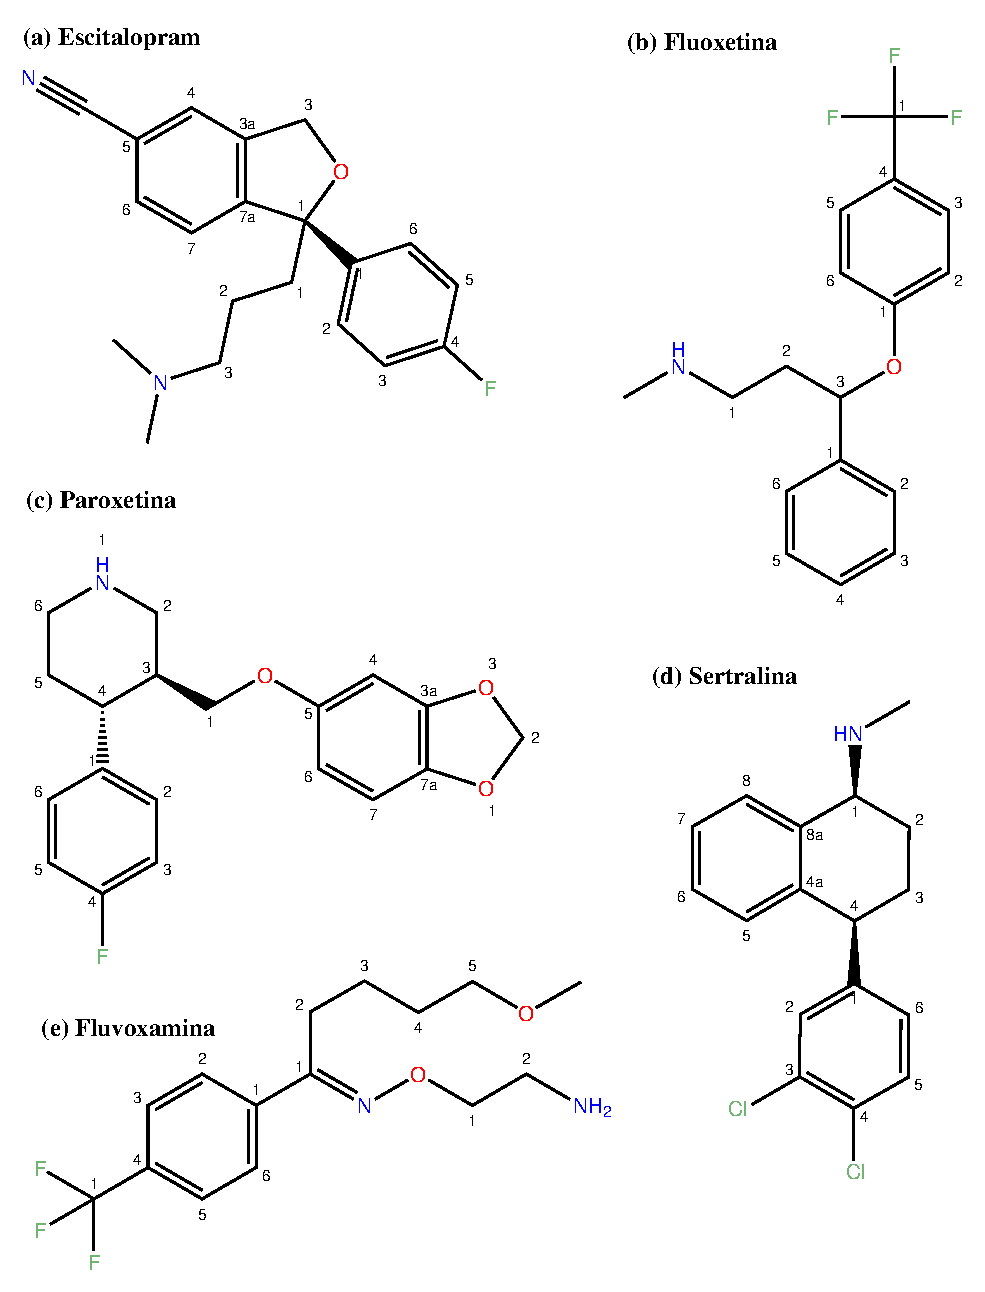
\includegraphics[scale=0.60]{Figuras/isrs.eps}
\caption{Estrutura química dos principais SSRIs comercializados. \cite{Schatzberg2015}} (adaptado)
\end{figure} 

\section{A fronteira da neurociência}

Na próxima década, grande parte dos atuais medicamentos já terão suas patentes expiradas, e darão lugar aos mecanismos mais promissores atualmente. Mediante tudo isso, mostra-se necessário a busca de novos fármacos seguros e eficazes, mas com mecanismos diferentes da antiga hipótese monoaminérgica.  \cite{Nestler2006}

\subsection{A hipótese do sistema de resposta imuno-inflamatório(IRS)}

A teoria das citocinas é certamente a fronteira na ajuda à pacientes com depressão grave. Desta forma, a associação entre inflamação e depressão fornecerá alvos importantes para o desenvolvimento de novos antidepressivos, podendo representar uma esperança a muitas pessoas. Durante vários anos, já vem sido estabelecido que citocinas pró-inflamatórias induzem não apenas sintomas de doenças inflamatórias, mas também estão presentes em transtornos depressivos graves. \cite{Dantzer2008}

\begin{figure}[H]
\centering
\includegraphics[scale=1]{Figuras/homeostase.png}
\caption{A depressão pode ser vista como consequência de um regime não homeostático de citocinas pro e anti-inflamatórias. \cite{Dantzer2008}}
\end{figure}

\section{Correlação entre Depressão e estresse oxidativo}

Em pacientes deprimidos, constata-se um aumento transitório na secreção de cortisol, como ocorre no estresse agudo, suprimindo o sistema imunitário e atrasando o processo anti-inflamatório. \cite{Kandel} Em geral, grande parte dos antidepressivos comercializados atuam sobre as monoaminas. Entre as áreas mais promissoras na pesquisa de antidepressivos, está os que possam agir no eixo hipotálamo-adrenal. Isto porque, especula-se que os sintomas de um episódio depressivo possa ser atribuído aos níveis elevados de cortisol. \cite{Schatzberg2015}

\subsection{Polimorfismos nos genes 5-HTTLPR e FKBP5}

  No decorrer da vida, eventos estressantes que envolvem ameaças, perdas ou humilhação, influenciam o início e o curso da depressão. No entanto, nem todas as pessoas que enfrentam situações difíceis decaem num episódio depressivo. Verificou-se que um polimorfismo funcional na região promotora do gene transportador de serotonina (5-HTTLPR) modera, em partes, a resiliência perante eventos estressantes ao longo da vida. Indivíduos com uma ou duas cópias do alelo curto do polimorfismo exibiram mais sintomas depressivos, depressão diagnosticável e suicídio em relação a indivíduos homozigotos para o alelo longo. \cite{Caspi2003}
  
  O impacto das alterações epigenéticas em FKBP5 estão em parte relacionadas à resistência e descontrole hormonal de glicocorticóides, reduzindo as respostas inflamatórias refletidas pela diminuição da sensibilidade
  ao glicocorticóide sintético dexametasona in vitro. \cite{Klengel2013}
  
\section{Processos inflamatórios e a Depressão}

O impacto do sistema inflamatório na ocorrência de depressão foi reconhecido pela primeira vez em meados de 1990. \cite{Yang2012} Quantidades crescentes de estudos sugerem que as respostas inflamatórias têm um papel importante na fisiopatologia da depressão. Verificou-se que os pacientes deprimidos apresentam níveis mais altos de citocinas pró-inflamatórias, proteínas de fase aguda, quimiocinas e moléculas de adesão celular. \cite{Raison2006} Esses achados sugerem que o direcionamento de citocinas pró-inflamatórias e suas vias de sinalização podem representar uma nova estratégia para o tratamento da depressão.

Quando comparados com indivíduos saudáveis, os pacientes clinicamente doentes com depressão maior exibem todas as características principais de processos inflamatórios, incluindo elevações nas citocinas inflamatórias relevantes e seus receptores solúveis no sangue periférico. \cite{Raison2009}

Também foram descritas associações entre sinais inflamatórios e sintomas depressivos individuais, como fadiga, atraso cognitivo e distúrbios do sono. Além do mais, processos inflamatórios também caracterizam-se por alterações no metabolismo de neurotransmissores, função neuroendócrina e plasticidade neural.\cite{Raison2009} 

Um grande estudo realizado em 2010 relata concentrações significativamente mais altas das citocinas pró-inflamatórias TNF-$\alpha$ e IL-6 em indivíduos deprimidos em comparação com o grupo controle. Embora resultados positivos e negativos venham sido relatados na literatura, esse resultado meta-analítico reforça as evidências de que a depressão é acompanhada pela ativação do sistema IRS. \cite{Dawlati2010}

Os níveis de duas citocinas, interleucina-6 (IL-6) e fator de necrose tumoral-$\alpha$ (TNF-$\alpha$) aumentaram de forma significativa em pacientes com estado grave de transtornos bipolares, depressivos e esquizofrenia em comparação com grupo controle. \cite{Miller2016}

As citocinas inflamatórias são nitidamente mais elevadas na depressão aguda e podem estar associadas à resistência ao tratamento monoaminérgico. Meta-análises confirmam níveis elevados de citocinas inflamatórias circulantes em pacientes deprimidos, e estudos longitudinais demonstraram que níveis elevados de citocinas séricas precedem sintomas depressivos. \cite{Kappelmann2018}

\begin{figure}[H]
\centering
\includegraphics[scale=1]{Figuras/immunitary_system.png}
\caption{Interações bioquímicas entre microglia-neurônio num cérebro saudável e condições homeostáticas, em comparação a um cérebro sob condições de estresse ou deprimido. \cite{Iwata2016}}
\end{figure}

\begin{table}[H]
\caption {Proteínas envolvidas em processos inflamatórios que podem ser de grande ajuda na busca de novos fármacos para o tratamento da depressão.\cite{Raison2009} (Adaptado)} 
    \begin{tcolorbox}[tab1,tabularx={XYYY},title= Alvos promissores do sistema inflamatório,boxrule=0.5pt]
    
    \centering{\textbf{Immune System} & \textbf{Central Nervous System}     &  \textbf{Neuroendocrine System}     &  \textbf{Autonomic Nervous System}}  \\ \hline \\
    
    \centering{Cytokines: \textit{TNF-alpha, IL-1, IL-6}   & Monoamines: \textit{5-HT, NE, DA} & HPA axis hormones: \textit{CRH, cortisol} & Catecholamines: \textit{alpha and beta adrenergic}}\\ \\
    
    \centering{Cytokine signalling: \textit{$NF-\kappa B$, MAPK} & IDO and its metabolites: \textit{KYN, QUIN, KA}  & HPA receptors: \textit{GR} & Parasympathetic outflow pathways: \textit{vagal nerve, alpha 7 and nAChR} }  \\
    
    \centering{Inflammatory mediators: \textit{COX-2, PG} & Extrasynaptic NMDA receptors}   \\ \\
    
    \centering{Reactive nitrogen/oxygen species: \textit{NO, $H_2O_2$}  &  Excitotoxic neurotransmitters: \textit{glutamate} & &} \\ \\
    
    \centering{Immune cells in the brain: \textit{microglia} & Neurotrophic factors: \textit{BDNF}}
    
    \end{tcolorbox}
\end{table}

A ativação de células T efetoras durante o estresse pode impedir o desenvolvimento de comportamentos depressivos e de ansiedade. Esses efeitos produzem células de resposta anti-inflamatória IL-4, que estimulam a produção de fatores de crescimento no cérebro que apoiam a neuroplasticidade e resiliência. \cite{Evolution2016} 

Vem sendo consolidado a visão de que processos imunológicos podem estar significativamente envolvidos na resposta ao tratamento em transtornos afetivos. \cite{Lanquillon2000}

\pagebreak\chapter{Objetivos}

\section{Objetivos específicos}

\chapter{Revisão Bibliográfica}

A grande maioria dos medicamentos, neutralizam a IL-6R mediante a interferência na ligação IL-6/gp80, afetando tanto a sinalização clássica quanto a trans-sinalização da IL-6. A proteína sgp130Fc, também denominada de sIL-6R subunidade $\beta$, bloqueia especificamente a trans-sinalização de IL-6 sem afetar a sinalização clássica. \cite{Simon2011} A forma solúvel de IL-6R (sIL-6R), que compreende o domínio extracelular do receptor, está envolvida em diversos processos pró-inflamatórios no organismo. \cite{Stefan2012} 

\section{Estrutura cristalográfica da interleucina sIL-6R subunidade $\alpha$}

Mediante a base de dados, Protein Data Bank(PDB), foram encontradas 8 estruturas proteicas expressas pelo ser humano(\textit{Homo sapiens}) que correspondem à palavra-chave: IL-6R. Os dois métodos de caracterização encontrados correspondem a NMR e XRD. No entanto, muitas estruturas estão incompletas por possíveis falhas na cristalização. Até o momento, existem apenas 2 estruturas com quantidade de resíduos superior a ($90\%$) pertencentes a uma região favorável no diagrama de Ramanchandran.

Para que haja a convicção de que o receptor é de fato a forma solúvel da proteína IL-R$\alpha$, foi realizada uma busca no catálogo da fabricante $Sigma-Aldrich$, onde a proteína recombinante sIL-R$\alpha$ possui o código $SRP3097$. Desta forma, por intermédio da ferramenta $Phyre2$ foi inserido a sequência de alinhamento de aminoácidos fornecido pela $Sigma-Aldrich$ no intuito de encontrar uma proteína homóloga, e portanto, a que será utilizada nesta pesquisa.     

\begin{figure}[H]
\centering
\includegraphics[scale=1.2]{Figuras/il6-ra.png}
\caption{Visualização estrutural por meio do software \textit{ICM-Browser} dos domínios extracelulares da proteína IL-6R(PDB ID: 1N26, cadeia $\alpha$), também denominado de sIL-6R. \cite{Varghese2002}}
\end{figure}

A proteína foi validada pela ferramenta RAMPAGE (Ramachandran Plot Investigation). Após a submissão do arquivo \texiit{.pdb}, a estrutura demonstrou que $90,6\%$ dos resíduos estavam presentes em uma região favorecida, embora outros $6,4\%$ dos resíduos compreenderam a área limite, e $3,0\%$ em condições de exceção. Mediante esses parâmetros, percebe-se uma excelente qualidade estrutural.

\begin{figure}[H]
\centering
\includegraphics[scale=0.6]{Figuras/ramachandran_1n26.png}
\caption{Análise estrutural da proteína sIL-6R mediante o mapa de Ramanchandran calculado por intermédio da ferramenta RAMPAGE. \cite{Ramanchandran2003}}
\end{figure}

\section{Sinalização clássica e trans-sinalização da interleucina-6}

A interleucina-6 é uma citocina não apenas envolvida nas respostas à inflamação e infecção, mas também na regulação de processos metabólicos, regenerativos e neurais. Em vários modelos, foi demonstrado que a sinalização clássica de IL-6 tem a função de mediar a ativação de vias anti-inflamatórias nas células-alvo. Em contraste, a trans-sinalização de IL-6 é observada em pacientes com doenças inflamatórias crônicas. \cite{Scheller2011}

A IL-6 tem uma ação dicotômica no CNC, exibindo propriedades neurotróficas, por um lado, e ações prejudiciais, por outro. Isso está de acordo com seu papel central na
neuroinflamação, que evoluiu como um processo benéfico, destinado a manter os tecidos em homeostase, mas que pode se tornar maligna quando em excesso. \cite{Spooren2011} Nesta perspectiva, é importante compreender os corretos mecanismos de inibição que possam trazer recuperação, ao invés de danos à saúde. A IL-6 é considerado uma proteína promissora para a intervenção clínica. Contudo, a sinalização que controla sua atividade é complexa, e distintas estratégias de intervenção podem inibir essa via. \cite{Jones2015}


\begin{figure}[H]
\centering
\includegraphics[scale=1]{Figuras/signalling_il6.png}
\caption{Vias de sinalização da interleucina-6. (a) Na sinalização clássica, emerge uma atividade anti-inflamatória. (b) Na trans-sinalização, emerge uma atividade pro-inflamatória. \cite{Johnson2018} (Adaptado)}
\end{figure}

\section{Triagem virtual baseada na similaridade estrutural}

Existem dois tipos principais de sistema de triagem virtual: as abordagens populares baseadas em estrutura, como docking e \textit{de novo}; Por outro lado, há abordagens mais simples, baseadas em ligantes, que são utilizadas como triagem inicial. No alicerce de qualquer sistema de triagem baseado em similaridade, está a medida usada para quantificar o grau de semelhança entre a estrutura de referência e cada uma das estruturas no banco de dados (real ou virtual) que está sendo rastreada. \cite{Willett2006}

A técnica de FP2(fingerprint 2D) vem sendo a representação mais adotada em triagens virtuais baseada em similaridade, não apenas por causa de sua eficiência computacional, mas também devido a sua eficácia demonstrada em muitos estudos comparativos. O FP2 consiste na codificação da estrutura de entrada em cadeias binárias. Dentre os coeficientes de similaridade usados para comparar fingerprints, o mais popular é o coeficiente de Tanimoto. \cite{Willett2006}
 
\begin{figure}[H]
\centering
\includegraphics[scale=1.2]{Figuras/vs_diversity.png}
\caption{Espectro estrutural dos inibidores de trombina, onde o grau de similaridade foi obtido pelo coeficiente de Tanimoto. \cite{Eckert2007}}
\end{figure}

\section{Triagem baseada nas propriedades físico-químicas(ADME)}

Os atuais esforços de química medicinal estão produzindo compostos com maior massa molecular e $c \log P$ do que medicamentos de décadas atrás. Os fármacos mais recentes, desde 1990, possuem $c \log P$ mediano de 3,1 e massa molecular de 432 Da. Embora a preocupação com perfis farmacocinéticos sejam importantes, no desenvolvimento de medicamentos, a toxicidade também é crucial. O carácter lipofílico($\log P$) é a propriedade molecular mais importante a ser considerada para reduzir o risco de toxicidade. \cite{Leeson2007}

\section{O surgimento da Mecânica Quântica}

Por muito tempo, químicos e físicos acreditavam que as regras que governam os sistemas microscópicos e macroscópicos eram semelhantes. Então, em 1900, Max Planck ofereceu uma proposta radical de que a radiação emitida pelo corpo negra estava limitada a certos valores discretos, ou seja, estava ``quantizada". À medida que o século XX avançava, tornou-se cada vez mais claro que a quantização era não apenas uma característica da luz, mas também das partículas fundamentais das quais a matéria é constituída.  \cite{Cramer2004}

Há um limite intrínseco à precisão de nossa capacidade de observação e a pequenez da perturbação que o acompanha, um limite que é inerente à natureza das coisas e que talvez nunca possa ser superado por uma técnica aprimorada ou por uma habilidade maior por parte do observador. A causalidade se aplica apenas a sistemas que não sofrem perturbações relativamente significativas, e assim, surge uma mecânica cuja visão é probabilística. \cite{Dirac1958}

Para descrever sistemas microscópicos, então, uma mecânica diferente foi necessária.
Um candidato promissor foi a mecânica das ondas, já que ondas estacionárias também são quantizadas, como proposto inicialmente por De Broglie. No entanto, descobriu-se também apresentar propriedades semelhantes a partículas. Para explicar essa dicotomia, uma nova mecânica, a mecânica quântica, foi desenvolvida. \cite{Cramer2004}

O operador que retorna a energia do sistema, $E$, possui um valor próprio sendo denominado de
operador Hamiltoniano, $\hat{H}$. Tem-se então, a equação de \textit{Schr\"{o}dinger} para o átomo de hidrogênio. \cite{Cramer2004}

\begin{equation}
    \hat{H} \Psi(r, R) = E \Psi(r, R)
\end{equation}

A forma típica do operador Hamiltoniano leva em conta cinco contribuições para a energia total de um sistema:
as energias cinéticas dos elétrons e núcleos, a atração dos elétrons para os núcleos, e as repulsões intereletrônicas e internucleares. \cite{Cramer2004}

\begin{equation}
    H = - \sum_{i} \cfrac{\hbar^2}{2m_e} \nabla_i^2 - \sum_{k} \cfrac{\hbar^2}{2m_k} \nabla_k^2 - \sum_i\sum_k \cfrac{e^2 Z_k}{r_{ik}} + \sum_{i < j} \cfrac{e^2}{r_{ij}} + \sum_{k < l} \cfrac{e^2 Z_k Z_l}{r_{kl}}
\end{equation}

Em geral, há muitas autofunções $\Psi$ aceitáveis para uma dada molécula, cada uma
caracterizada por um autovalor associado $E$ distinto. Desta forma, existe um conjunto completo (talvez infinito) de $\Psi_i$ com autovalores $E_i$. Para facilitar uma manipulação futura, podemos assumir sem perda de generalidade de que essas funções de onda são ortonormais, isto é, para um sistema contendo uma única partícula, a função de onda depende de apenas três coordenadas: \cite{Cramer2004}

\begin{equation}
    \int \int \int \Psi_i \Psi_j dx dy dz = \delta_{ij}
\end{equation}

\begin{equation}
    \int \Psi_j H \Psi_i dr = E_i \delta_{ij}
\end{equation}

É importante destacar que a $Eq.(3.4)$ é crucial na determinação da energia molecular de um sistema. Todavia, a natureza real da função de onda e da solução exata da integral na $Eq.(3.4)$ é complexa e abstrata para uma analogia intuitiva. \cite{Cramer2004}

\subsection{O princípio variacional}

Será discutido os modelos físicos em sistemas moleculares de muitos corpos. Isto porque, funções de onda exatas para esses sistemas são extremamente difíceis de expressar porque os movimentos correlacionados de partículas possuem uma complexidade matemática muito alta. Sendo assim, para definir o estado fundamental de um sistema, podemos julgar a qualidade das funções de onda mediante suas energias associadas, de maneira a ser buscado o valor mínimo de energia do sistema ou estado de equilíbrio. \cite{Cramer2004}

Esse resultado é crítico porque nos mostra que não precisamos construir a suposta função de onda $\Psi$ como uma combinação linear de funções de onda ortonormais $\Psi_i$ (desconhecidas), mas podemos construí-la de várias maneiras distintas. \cite{Cramer2004}

\begin{equation}
    \Phi = \sum_i c_i \Psi_i
\end{equation}

\begin{equation}
    \int \Phi H \phi dr - E_0 \int \Phi^2 dr \geq 0
\end{equation}

\begin{equation}
     \cfrac{\mathlarger{\int} {\Phi H \Phi dr}}{\mathlarger{\int}{\Phi^2 dr}} \geq E_0
\end{equation}

A qualidade da aproximação será determinada pelo quão baixo for o valor calculado para a integral na $Eq. (3.7)$. Além disso, como precisamos encontrar as menores energia possíveis dentro das restrições de como construímos uma função de onda, pode-se usar todas as ferramentas que o Cálculo Diferencial e Integral disponibiliza para localizar valores extremos. \cite{Cramer2004}

\subsection{Aproximação de Born-Oppenheimer}



\subsection{Aproximação de Hartre-Fock}

\subsection{Teoria do Funcional da Densidade(DFT)}

\subsection{Funções de Base}

\subsection{Funcionais de Troca e Correlação}

\section{Docking Molecular}

Nos esforços da descoberta de medicamentos, é fundamental a compreensão dos mecanismos pelos quais os receptores de proteínas numa patologia reconhecem e interagem com os substratos moleculares ou inibidores. Apesar dos grandes avanços nos algoritmos de docking molecular nas últimas décadas, ainda existem muitas lacunas. Em particular, a ausência da flexibilidade de proteínas tem um aspecto crítico para uma melhor compreensão dos princípios que orientam a interações entre ligantes e proteínas. \cite{Souza2006}

A questão principal de todos os programas de docking é abordar qual combinação de orientação e conformação (pose) é a mais favorável em relação a todas as outras combinações possíveis(confôrmeros). Quando aplicado à triagem virtual, o processo também exige uma comparação da melhor conformação de um determinado ligante com a de outros possíveis ligantes, de modo que um pontuação(score) possa ser obtida. \cite{Perola2004}

Os softwares de docking molecular executam um algoritmo de busca no qual a conformação do ligante é avaliada recursivamente até que a convergência para a energia mínima seja alcançada. Finalmente, uma função de pontuação de afinidade, $\Delta G$ [U total em kcal / mol], é empregada para classificar as orientações mais favoráveis para a soma das energias eletrostática e van der Waals. \cite{Pagadala2017}

\begin{equation}
    N_{conf} = \prod^{N}_{i=1} \prod^{n_{inc}}_{j=1} \cfrac{360º}{\theta_{i, j}}
\end{equation}

Em uma busca conformacional sistemática, a $Eq.(3.8)$ fornece o número de possíveis conformações moleculares pelos seguintes parâmetros: $N$ é o número de ligações rotacionáveis e $\theta_{i, j}$ é o valor do incremento do ângulo de rotação $j$ da ligação $i$.\cite{Kitchen2004}

\subsection{Algoritmos de Busca}

Um rigoroso algoritmo de pesquisa elucidaria todos os modos de ligação possíveis entre o ligante e o receptor. Desta forma, consideraria todos os graus de translação e liberdade rotacional do ligante, como também os graus de liberdade conformacionais da proteína. No entanto, \cite{Taylor2002}

\subsection{Algoritmos Genéticos(GA) de busca}

Os genótipos são mapeados para fenótipos por uma função de mapeamento de desenvolvimento. Ao atingir iterações suficientes da pesquisa local a ponto de encontrar o mínimo local, uma função de mapeamento inverso é usada para converter seu fenótipo em seu genótipo correspondente. No docking molecular, a pesquisa local é realizada pela conversão contínua do genótipo para o fenótipo.

O estado do ligante corresponde ao genótipo, enquanto suas coordenadas atômicas correspondem ao fenótipo. No encaixe molecular, a afinidade é a energia total de interação do ligante com a proteína. O cromossomo é composto de uma sequência de genes de valor real: três coordenadas cartesianas para a tradução do ligante; quatro variáveis que definem um quatérnion especificando a orientação do ligante; e um valor real para cada torção do ligante, respectivamente. 

No desenvolvimento do AutoDock Vina, diversas abordagens estocásticas de otimização global foram exploradas, incluindo algoritmos genéticos. No algoritmo, há uma sucessão de etapas que consistem em uma mutação e uma otimização local, sendo cada etapa aceita de acordo com o critério de Metropolis. Durante a implementação, foi adotado o método Broyden-Fletcher-Goldfarb-Shanno(BFGS) para a otimização local, que é um eficiente método quasi-Newton. \cite{Vina2010}

\begin{figure}[H]
\centering
\includegraphics[scale=1.35]{Figuras/lga_search.png}
\caption{É ilustrado o algoritmo de busca Lamarckiano(LGA), assim como a busca de um mínimo local mediante a conversão e mutação recursiva entre genótipos e o respectivo fenótipo. \cite{Autodock1998}}
\end{figure}

\subsection{Algoritmos de Scoring}

Num campo de força AMBER utilizado nos softwares AutoDock(1998) e AutoDock Vina(2010), para dois átomos $i, j$, a energia atômica em pares é avaliada pela soma das interações de van der Waals, ligações de hidrogênio, energia de Coulomb e dessolvatação. \cite{Autodock1998} A função de score do AutoDock 4 foi calibrada a partir de 30 dados experimentais de proteínas em complexo. A implementação tem como base o ciclo termodinâmico de Wesson-Eisenberg.\cite{Autodock1998} No AutoDock Vina, a função de score é uma combinação de abordagem empírica, devido à calibração por meio de 1300 complexos proteicos, e baseada no conhecimento físico-químico das interações proteína-ligante. \cite{Vina2010}

\begin{equation}
    \Delta G_{obs} = RT \ln {K_i}
\end{equation}

A calibração da função de scoring foi a partir de valores experimentais de $\Delta G$, onde $K_i$ representa a constante de inibição. \cite{Autodock1998}

\begin{equation}
    \Delta G_{binding} = \Delta G_{vdW} + \Delta G_{elec} + \Delta G_{hbond} + \Delta G_{desolv} + \Delta G_{tors}
\end{equation}

$\Delta G_{vdW} \rightarrow$ Representa o potencial de Lennard-Jones para dispersão e repulsão intereletrônica; \\

$\Delta G_{elec} \rightarrow$ Efeitos eletrostáticos baseados no modelo dielétrico de Solmajer \& Mehler; \\

$\Delta G_{hbond} \rightarrow$ Potencial das ligações de hidrogênio conforme o modelo da direcionalidade de Goodford's; \\

$\Delta G_{desolv} \rightarrow$ Dessolvatação por meio do emparelhamento de Stouten; \\

$\Delta G_{desolv} \rightarrow$ Energia livre associada às ligações rotacionáveis. \\

A $Eq. (3.11)$ representa o modelo físico utilizado pelo AutoDock4 como função para estimar a energia livre total entre receptor-ligante: \cite{Autodock1998}

\begin{equation}
\begin{split}
       V = W_{vdw} \sum_{i,j} \left( \cfrac{A_{ij}}{r_{ij}^{12}} - \cfrac{B_{ij}}{r_{ij}^6} \right) + W_{hbond} \sum_{i,j} E(t) \left(  \cfrac{C_{ij}}{r_{ij}^{12}} - \cfrac{D_{ij}}{r_{ij}^{10}}    \right) + W_{elec} \sum_{i,j} \cfrac{q_i q_j}{\epsilon(r_{ij}) r_{ij}} + \\ W_{sol} \sum_{i, j} (S_i V_j + S_j V_i) e^{(-r_{ij}^2/2\sigma^2)}
\end{split}
\end{equation}

\section{Avaliação dos resultados de docking}

Existem dois modos de RMSD: O RMSD absoluto e o RMSD relativo. O RMSD absoluto mede a distância entre pares de átomos correspondentes sem translação ou rotação de coordenadas. Entretanto, o RMSD relativo implica uma etapa de alinhamento(simetrização) adicional do moléculas antes do cálculo RMSD real. \cite{Kirchmair2008}

\begin{equation}
    <RMSD_{lb}(c1, c2)> = max(rmsd'(c1, c2), rmsd'(c2, c1))
\end{equation}

\begin{equation}
    <RMSD'_{ab}> = \sqrt{\cfrac{1}{N} \sum_{i} min_{j} r_{ij}^2}
\end{equation}

A precisão das \textit{poses} de encaixe é quantificada pelo cálculo do RMSD entre o valor experimental da estrutura ligante determinada e a calculada pelo algoritmo de busca. Atualmente, o RMSD entre uma pose de encaixe gerada e a conformação experimental do ligante representa a referência mais estabelecida para o sucesso do algoritmo de predição da conformação. \cite{Kirchmair2008} O valor de corte RMSD de $2 \si{\angstrom}$  é frequentemente usado como critério da validade de predição do docking proteína-ligante. \cite{Bursulaya2003} 

\section{Teorias de interação proteína-ligante}

A teoria \textit{``chave-fechadura''} proposta por \textit{Fisher} em 1894, considerava o receptor rígido e imóvel ancorando em um ligante sem sofrer quaisquer rearranjos conformacionais(conformação reativa). Em contrapartida, foi largamente abandonada em favor de modelos de ligação que não apenas consideram alterações conformacionais, mas também um ajuste estocástico de receptores e ligantes. \cite{Durrant2011} Desta forma, o encaixe induzido(em termos modernos, desestabilização do estado fundamental) advém da teoria do estado de transição, a hipótese de complementaridade enzima-ligante. \cite{Benkovic2003}

\begin{figure}[H]
\centering
\includegraphics[scale=0.35]{Figuras/induced_fit2.png}
\caption{Inibidores da proteína FKBP51 interagem pelo mecanismo de encaixe induzido, causando mudanças conformacionais no complexo receptor-ligante.  \cite{Gaali2015}}
\end{figure}

\section{Limitações dos algoritmos de docking}

A maior limitação dos métodos de docking é o modelo rígido do receptor. O AutoDock e o AutoDock Vina permitem flexibilidade limitada das cadeias laterais do receptor. Para sistemas com movimentos maiores de loops ou domínios, uma variedade de conformações do receptor pode ser calculada mediante dinâmica molecular e, em seguida, realizam-se simulações de docking a partir de snapshots. \cite{Autodock2016}

A água desempenha um papel crítico na termodinâmica da interação receptor-ligante. A contabilização exata dos efeitos da solvatação/dessolvatação ainda permanece um desafio significativo. \cite{Yuriev2015}



\pagebreak\chapter{Metodologias}

Neste capítulo serão apresentados os conceitos para compreensão das ferramentas computacionais. Será feito um estudo dos métodos e teorias já estabelecidos na literatura para os cálculos de estrutura eletrônica e docking molecular juntamente com seus parâmetros técnicos. Todavia, uma descrição com maior rigor matemático e detalhamento pode ser encontrado nas seguintes leituras adicionais. 

\section{Otimização estrutural e análise conformacional}

Conforme a geometria ao qual o candidato à fármaco inibidor interage com a proteína receptora, pode-se, haver ou não, bioatividade. Desta forma, uma análise conformacional mostra a estereoquímica das diferentes orientações espaciais de um futuro medicamento. Sendo assim, será rotacionado os ângulos diedrais das ligações químicas, possibilitando a visualização das orientações mais energeticamente favoráveis ao fármaco, denominados de confôrmeros. \cite{Kiametis2012}

Contudo, durante a geração dos confôrmeros podem haver distorções nos comprimentos das ligações, como também, variações nos ângulos de torção. Sendo assim, as conformações mais estáveis são obtidas por otimização de geometria mediante cálculos de mecânica molecular ou mecânica quântica. \cite{Silva2017}

A pré-otimização dos ligantes será efetuada por métodos mecânico-quânticos, de natureza semi-empírica mediante o software open-source: \textit{GAMESS(US) na versão Junho 2019 R1 em arquitetura Linux x64 bits}. Optou-se pelo halmitoniano não relativístico Parametric Method Number 6(PM6). Devido aos limites computacionais, escolheu-se inicialmente um método semi-empírico por apresentar menor tempo de processamento comparado a métodos \textit{ab initio}. Todavia, os resultados obtidos de forma semi-empírica possuem menor exatidão com a realidade.

Os valores de energia são obtidos a partir de uma versão modificada da equação de $Schr\"{o}dinger$ para fenômenos de muitos corpos. A partir da análise conformacional será construído um gráfico para a superfície de energia potencial(PES), crucial na determinação da conformação de maior estabilidade em cada par de ângulos diedrais. 

Ainda será preciso uma reotimização dos ligantes, com o intuito de aumentar a precisão dos mínimos de energia. A reotimização será mediante cálculos \textit{ab initio} por meio do pacote computacional: \textit{GAMESS(US)}. A pré-otimização contribui na redução do tempo de processamento durante os cálculos \textit{ab-initio}. Em relação aos parâmetros, escolheu-se o modelo Restricted Hartre-Fock(RHF) com funções de base gaussianas do tipo $6-311G** +(2d,p)$. O motivo das especificações teóricas serão descritas detalhadamente ao longo deste capítulo.



\pagebreak\input{./06_Perspectives/6.1_results}

%\bibliographystyle{unsrt}
%\begin{thebibliography}{00}

    \bibitem{1} Charney, Dennis S.; Neurobiology of mental illness - 4th edition. Oxford University Press, 2013. p.496
    
    \bibitem{2} Wong, M.L., \& Licinio, J. (2004). From monoamines to genomic targets: A paradigm shift for drug discovery in depression. \textbf{Nature Reviews Drug Discovery}, Vol.3, pp. 136-151.
    
    \bibitem{3} Tacchi, Mary Jane; \& Scott, Jan; Depression: A very short introduction - 1th edition. Oxford University Press, 2017. p.91
    
    \bibitem{4} Nemeroff, C.B., \& Vale, W. W. (2005). The neurobiology of depression: inroads to treatment and new drug discovery. \textbf{Neurobiology of Depression}, Vol. 66.
    
    \bibitem{5}
    
    \bibitem{6} Stahl, Stephen M.; Psicofarmacologia: bases neurocientíficas e aplicações práticas - 4ª edição. GEN, 2014. p.
    
    \bibitem{7} Jeon, S. W., \& Kim, Y. K. (2016). Molecular neurobiology and promising new treatment in depression. \textbf{International Journal of Molecular Sciences}, 17(3).
    
    \bibitem{8} Krishnan, V., \& Nestler, E. J. (2008). The molecular neurobiology of depression. \textbf{Nature}, Vol. 455, pp.894-902.
    
    \bibitem{9} Yanik, M., Erel; \& Erel, O.; \& Kati, M. (2004). The relationship between potency of oxidative stress and severity of depression. \textbf{Acta Neuropsychiatrica}, 16(4), 200-203.
    
    \bibitem{10} Schatzberg, Alan F. Manual de psicofarmacologia clínica. - 6ª edição. Artmed, 2009. p.58
    
    \bibitem{11} Ciraulo, Domenic A. [et al.]; Pharmacotherapy of Depression - 2th edition. Humana Press, 2011. p.
    
    \bibitem{12} Belmaker, R.H.; \& Agam, Galila. (2008). \textbf{The New England Journal of Medicine.} Vol.358, p.55-68.   
    
    \bibitem{13} Richards, C. Steven; O'Hara, Michael W. (2014). The Oxford Handbook of Depression and Comorbidity. Oxford University Press. p. .
    
    \bibitem{14} American Psychiatric Association (2013), Diagnostic and Statistical Manual of Mental Disorders - 5th edition. Arlington: American Psychiatric Publishing, pp. 165.
    
    \bibitem{15} Stein, Dan J.; \& Kupfer, David J. [et al.]. Textbook of mood disorders. (2006). American Psychiatric Publishing - 1st edition. p.38
    
    \bibitem{16} Kiametis, Alessandra Sofia. Modelagem molecular de potenciais candidatos a inibidores da acetilcolinesterase. 76 f., il. Tese(Doutorado em Física) — Universidade de Brasília, Brasília, 2012.
    
    \bibitem{17} Silva, Mônica de Abreu. Modelos preditivos baseados em descritores moleculares e modos de interação receptor-ligante para inibidores de Acetilcolinesterase. 143 f., il. Tese(Doutorado em Física) - Universidade de Brasília, Brasília, 2017.
    
    \bibitem{18} Berton, O. \& Nestler, E.J. New approaches to antidepressant drug discovery: beyond monoamines. \textbf{Nature Reviews Neuroscience.} v.7, pp.137-151 (2006). 
    
    \bibitem{19} Nestler, E.J. (et al.) Treatment resistant depression: A multi-scale, systems biology approach.
                 \textbf{Neuroscience & Biobehavioral Reviews}, v.84, pp.272-288 (2018).
                 
    \bibitem{20} Bissete, Garth [et al.] Elevated Concentrations of CRF in the Locus Coeruleus of Depressed Subjects. \textbf{Nature Neuropsychopharmacology}, v.28, pp.1328-1335 (2003).
    
    \bibitem{21} Ramachandran, K.I. [et al.] Computational Chemistry and Molecular Modeling. Springer Publishing, (2008), pp.37
    
    \bibitem{22} Durrant, J.D. \& McCammon, J.A. Molecular dynamics simulations and drug discovery. \textbf{BMC Biology}, v.9, pp.71 (2011).
    
    \bibitem{23} Kishimoto, T. [et al.]. Single-dose infusion ketamine and non-ketamine N-methyl-d-aspartate receptor antagonists for unipolar and bipolar depression: A meta-analysis of efficacy, safety and time trajectories. \textbf{Psychological Medicine}, v.46 (7), pp.1459-1472 (2016)
    
\end{thebibliography}

\clearpage
\pagestyle{references}
\label{References}
\renewcommand{\bibname}{Referências}
\addcontentsline{toc}{chapter}{\normalsize\textbf{REFERÊNCIAS}}
\bibliographystyle{acm}
\bibliography{research} 

\clearpage
\pagestyle{timeline}
\pagebreak
% code by Andrew:
% http://tex.stackexchange.com/a/28452/13304
\makeatletter
\let\matamp=&
\catcode`\&=13
\makeatletter
\def&{\iftikz@is@matrix
  \pgfmatrixnextcell
  \else
  \matamp
  \fi}
\makeatother

\newcounter{lines}
\def\endlr{\stepcounter{lines}\\}

\newcounter{vtml}
\setcounter{vtml}{0}

\newif\ifvtimelinetitle
\newif\ifvtimebottomline
\tikzset{description/.style={
  column 2/.append style={#1}
 },
 timeline color/.store in=\vtmlcolor,
 timeline color=red!80!black,
 timeline color st/.style={fill=\vtmlcolor,draw=\vtmlcolor},
 use timeline header/.is if=vtimelinetitle,
 use timeline header=false,
 add bottom line/.is if=vtimebottomline,
 add bottom line=false,
 timeline title/.store in=\vtimelinetitle,
 timeline title={},
 line offset/.store in=\lineoffset,
 line offset=6pt,
}

\NewEnviron{vtimeline}[1][]{%
\setcounter{lines}{1}%
\stepcounter{vtml}%
\begin{tikzpicture}[column 1/.style={anchor=east},
 column 2/.style={anchor=west},
 text depth=0pt,text height=1ex,
 row sep=1ex,
 column sep=1em,
 #1
]
\matrix(vtimeline\thevtml)[matrix of nodes]{\BODY};
\pgfmathtruncatemacro\endmtx{\thelines-1}
\path[timeline color st] 
($(vtimeline\thevtml-1-1.north east)!0.5!(vtimeline\thevtml-1-2.north west)$)--
($(vtimeline\thevtml-\endmtx-1.south east)!0.5!(vtimeline\thevtml-\endmtx-2.south west)$);
\foreach \x in {1,...,\endmtx}{
 \node[circle,timeline color st, inner sep=0.15pt, draw=white, thick] 
 (vtimeline\thevtml-c-\x) at 
 ($(vtimeline\thevtml-\x-1.east)!0.5!(vtimeline\thevtml-\x-2.west)$){};
 \draw[timeline color st](vtimeline\thevtml-c-\x.west)--++(-3pt,0);
 }
 \ifvtimelinetitle%
  \draw[timeline color st]([yshift=\lineoffset]vtimeline\thevtml.north west)--
  ([yshift=\lineoffset]vtimeline\thevtml.north east);
  \node[anchor=west,yshift=16pt,font=\large]
   at (vtimeline\thevtml-1-1.north west) 
   {\textsc{Timeline \thevtml}: \textit{\vtimelinetitle}};
 \else%
  \relax%
 \fi%
 \ifvtimebottomline%
   \draw[timeline color st]([yshift=-\lineoffset]vtimeline\thevtml.south west)--
  ([yshift=-\lineoffset]vtimeline\thevtml.south east);
 \else%
   \relax%
 \fi%
\end{tikzpicture}
}

\footnotesize
\justify
\begin{vtimeline}[description={text width=8.4cm},
 row sep=16ex, 
 timeline color=cyan!80!blue,
 timeline title={Cronograma proposto ao andamento da pesquisa.}]


 
\textcolor{blue!30!green!75}{Agosto(2020)} $\rightarrow$ \textcolor{gray}{Julho(2021)} & Levantamento bibliográfico sobre as hipóteses centrais do Transtorno Depressivo. Avanços na literatura entre as ferramentas de otimização, triagem virtual, ADME e docking molecular.  \endlr

\textcolor{gray}{Agosto(2020)} $\rightarrow$ \textcolor{gray}{Setembro(2020)}   & Triagem virtual baseada na similaridade espacial com os inibidores consolidados de \textit{IL-6R}. Seleções dos inibidores que obedecem à Regra de Lipinski. Otimização e estudo dos descritores moleculares. \endlr

\textcolor{gray}{Outubro(2020)} $\rightarrow$ \textcolor{gray}{Janeiro(2020)}  & Preparação do receptor \textit{IL-6R} mediante protonação por adição de Hidrogênio e cargas parciais. Estudos de docking do tipo semirrígido-flexível nos softwares AutoDock Vina e GOLD.\endlr

\textcolor{gray}{Fevereiro(2021)} $\rightarrow$ \textcolor{gray}{Abril(2021)}  & Revisão e possíveis correções de todos os cálculos efetuados e análise comparativa com pesquisas já consolidadas na literatura. \endlr

\textcolor{gray}{Maio(2021)} $\rightarrow$ \textcolor{gray}{Junho(2021)} &  Análise das conclusões, estudo dos mecanismos de síntese dos fármacos mais promissores e perspectivas futuras. \endlr

\textcolor{gray}{Junho(2021)} $\rightarrow$ \textcolor{gray}{Julho(2021)} & Predição da probabilidade de interações com outras proteínas no organismo. Considerações éticas sobre o tratamento psicofarmacológico. \endlr

\textcolor{gray}{Julho(2021)} & Elaboração do resumo e relatório final de Iniciação Científica. \textcolor{red!80}{(atividade obrigatória)}  \endlr

\textcolor{gray}{Julho(2021)} & Preparação da apresentação final para o Congresso de Iniciação Científica. \textcolor{red!80}{(atividade obrigatória)} \endlr
\end{vtimeline}

\addcontentsline{toc}{chapter}{\normalsize\textbf{CRONOGRAMA}}

%\printindex    %Removi o índice remissivo para a versão oficial do trabalho.

\end{document}